\documentclass[xcolor=svgnames,handout]{beamer}

\usepackage[utf8]    {inputenc}
\usepackage[T1]      {fontenc}
\usepackage[english] {babel}

\usepackage{amsmath,amsfonts,graphicx}
\usepackage{beamerleanprogress}
\usepackage{verbatim}


\title
  [Triaging Bugs\hspace{2em}]
  {Triaging Software Bugs}

\author
  [Matile, Steiner]
  {Raphael Matile\quad Yves Steiner}

\date
  {December 15, 2016}

\institute
  {Big Data and Business Analytics}


\begin{document}

\maketitle

\section
  {Introduction}

\begin{frame}
  {Introduction}

  Steps considered in the process of creating the prediction model\pause

  \begin{itemize}
  \item System setup and technologies \pause
  \item Preparing the data\pause
  \item Considered prediction variables\pause
  \item Results of regressions\pause
  \item Conclusion
  \end{itemize}
\end{frame}

\section
  {Technologies}

\begin{frame}
  {System setup/technologies}

Used technologies to create this model:\pause

  \begin{itemize}
  \item Python3.5 \pause
  \item Numpy \pause
  \item SQLite3 \pause
  \item scikit-learn (linear models) \pause
  \item Keras and Theano (neural net)
  \end{itemize}
  
\end{frame}

\section{Dataset}
\begin{frame}
  {Dataset}
  Mozilla and Eclipse Defect Tracking Dataset (MSR 2013)\footnote{\url{https://github.com/ansymo/msr2013-bug_dataset}} \bigbreak
 
  Contains information about: 
  \begin{itemize}
      \item Current status
      \item Assigned Priority
      \item ...
  \end{itemize}
  \bigbreak
    Includes incremental modifications of each bug
  
\end{frame}

\section{Preparing the data}
\begin{frame}
  {Preparing the data}

The data was derived from the 
two CSV files required some reformatting in order to import them into the database. The \texttt{CC} and the \texttt{short-desc} file.

\end{frame}


\begin{frame}[fragile]
  {Preparing the data - CC-file}
  The CC file had multiple items separated by a comma for the \texttt{what} column, this resulted in a file reading error since it created more than the expected four columns. We used the following code to format the CSV file:
 \begin{verbatim}
        for row in reader:
            length_row = len(row)
            str = row[1]
            if length_row > 4:
                for x in range(2, 2 + length_row - 4):
                    str = str + ',' + row[x].strip()
                row[1] = str
                row[2] = row[2 + length_row - 4]
                row[3] = row[3 + length_row - 4]
                for x in range(0,length_row-4):
                    del row[-1]
 \end{verbatim}
\end{frame}

\begin{frame}[fragile]
  {Preparing the data - Remaining Files}
To import the CSV data into our database we used a regular expression, which captured the groups: id, what, timestamp, who

\bigbreak

\begin{verbatim}
([0-9]+),((?:.|(?:\n\t)+)*),([0-9]+),([0-9]+)
\end{verbatim}


\end{frame}

\begin{frame}
  {Preparing the data - Training, Validation, Test Set}

  In order to create valid models, we set up the database with the given data and split it up into train (50\%), validation (25\%) and test (25\%) sets.
  \bigbreak
  The validation set is currently only used for training the neural network
  
\end{frame}

\section{Prediction Variables}
\begin{frame}
  {Considered prediction variables\footnote{These prediction variable are all chosen from the list of the use case.}}

  \begin{enumerate}
      \item Success Rate of a bug assignee
      \item Success Rate of a bug reporter
      \item Success Rate of a bug report for every reporter-assignee pair
      \item Success Rate of a bug in terms of how many times it got reassigned
       \item Success Rate for number of reassignments of a bug
       \item The duration in seconds of how long a bug was opened
       \item Success Rate of the component to which the bug was assigned
       \item Success Rate of a bug considering the reporter and all names on the CC 
       \item Success Rate of the software version to which the bug was assigned
  \end{enumerate}
  
\end{frame} 

\begin{frame}{Considered prediction variables - Success}
  In order to determine if a bug was successful or failed, we defined the following combinations of \texttt{current\_status} and \texttt{current\_resolution} for a report as a success:\\
  \begin{table}[]
\centering
\begin{tabular}{cc}
\textbf{current status} & \textbf{current resolution} \\ \hline 
RESOLVED                 & WORKSFORME                   \\
RESOLVED                 & FIXED                        \\
VERIFIED                 & FIXED                        \\
CLOSED                   & WORKSFORME                   \\
CLOSED                   & FIXED    
\end{tabular}
\end{table}
\end{frame}

\begin{frame}{Considered prediction variables - Fail}
  The following combinations of \texttt{current\_status} and \texttt{current\_resolution} are considered as a fail:\\
  \begin{table}[]
\centering
\label{my-label}
\begin{tabular}{cc}
\textbf{current status} & \textbf{current resolution} \\ \hline
RESOLVED                 & WONTFIX                      \\
RESOLVED                 & INVALID                      \\
CLOSED                   & WONTFIX                      \\
CLOSED                   & INVALID                      \\
VERIFIED                 & WONTFIX                      \\
VERIFIED                 & INVALID
\end{tabular}
\end{table}              
\end{frame}

\section
  {Results of regressions}

\begin{frame}
  {Results of regressions}

After calculating the prediction variables we've run different prediction  models in order to determine their performance:

\begin{table}[]
\centering
\label{my-label}
\begin{tabular}{lcc}
\multicolumn{1}{c}{\textbf{Model}} & \textbf{Accuracy}                 & \multicolumn{1}{l}{\textbf{f1-Score}} \\ \hline
Classic linear regression          & 0.751108192415                    & 0.836567485985                        \\
Lasso linear regression            & 0.731012969956                    & 0.826300835418                        \\
Logistic regression                & 0.752290264324                    & 0.836625086625                        \\
Bayesian ridge regression          & 0.751108192415                    & 0.836574533224                        \\
Decision tree                      & 0.907273025776                    & 0.92358480355                         \\
Neural Netowrk                     & 0.652963388606                    &   0.790051846408                       \\
Optimized Neural network\footnote{Uses the first 120000 entries as training, the last 30000 as test set}                     & \multicolumn{1}{l}{0.81037282411} & \multicolumn{1}{l}{0.81037282411}    
\end{tabular}
\end{table}

\end{frame}


\begin{frame}
  {ROC Curves}

  \begin{figure}[t]
    \centering
    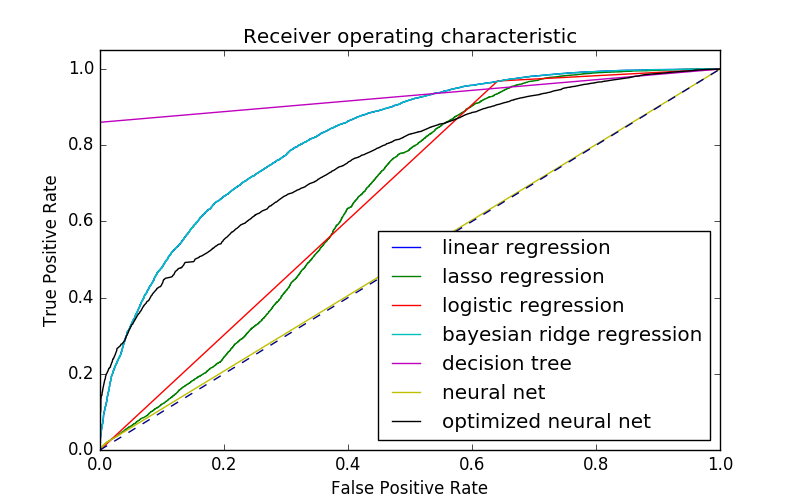
\includegraphics[height=\dimexpr11\textheight/16\relax]{resources/roc_curves}
    \caption{ROC Curves for different validated models}
  \end{figure}
\end{frame}


\section
  {Conclusion}
\begin{frame}
    {Conclusion}
    
    Surprisingly, the decision tree achieved the best score over all models. Looking at its structure\footnote{Included in the submitted code repository}, its dimensions can indicate a certain grade of overfitting to the data. However, cross-validation showed, that different folds result in completely different accuracies.
    \bigbreak
    Also, the optimized neural network, which uses the first 120000 entries of the total set, indicates that there is a structure given in the dataset, resulting in quite different results, when shuffled.
    
\end{frame}

\end{document}

